\chapter{Field Test}

In order to test the rover's ability to localize itself, a simple field test was conducted in a parking lot. Inspiration for this experiment comes from Moore and Stouch \cite{robot_localization_paper}.

\section{Experiment Design}

The rover was initially placed in a parking lot oriented facing west. It was then driven in a roughly rectangular shape around the lot using the virtual\_joystick node, described in section \ref{sectionJoystick}. During this time the raw sensor data streaming in from the Arduino and phone was recorded and saved into a ROS bag file. The rover was driven in a loop, such that its initial and ending position and orientation were roughly equal. Total collection time was five and a half minutes.

See Figure \ref{fig:roverPath} for two representations of the path taken. Figure \ref{figRouteMemory} displays the path actually traversed, while Figure \ref{figRouteGPS} is constructed from the phone's GPS readings. At no point did the rover go onto the grass.

The ROS \textit{rosbag} utility was then used to repeatedly simulate the recorded sensor messages, while the EKF was run in different configurations. The rover's state was computed from raw wheel odometry, from wheel odometry fused with the IMU data, and from wheel odometry, IMU data, and GPS fixes all fused together. Refer to Table \ref{tab:configs} for a review of which state variables each sensor affects.

\section{Results}

% laptop had no problem computing using the filter. No memory spikes either. Very computationally efficient! laptop is enough for localization - is it enough for navigation?

During each filter computation, a state estimate was produced at 30 Hz in a local frame, and that output was then transformed into a global frame, where position is given as latitude and longitude. These gps coordinates were then plotted using the handy GPS Visualizer tool \cite{gps_visualizer}. Figure \ref{fig:ekfOutputs} displays those plots.

Figure \ref{figRouteOdom} shows the estimated path when fusing only the wheel encoder output. The initial upward trajectory and left turn are tracked reasonably well, but the second left turn rotates too far and throws the rest of the estimate off.

Figure \ref{figRouteOdomImu} shows the path generated when fusing wheel odometry with IMU data. In this case the shape of the path is much closer to truth, though the initial right turn is under-estimated.

Lastly, Figure \ref{figRouteOdomImuGps} shows the result of fusing both previous sensors with GPS fixes. This plot looks much like the raw gps plot in Figure \ref{figRouteGPS}, however upon close inspection one can see jagged jumps in position. These jumps are instantaneous and actually lead to a discontinuous position estimate, though the visualizing tool connects every point. They are caused by the filter instantaneously adjusting the position estimate based on an incoming gps fix. The filter does give weight to the current estimate, so the new adjusted position lies in between the gps fix and the old position estimate. Due to the frequent gps fixes and slow velocity of the rover, the estimated path does not vary too far from the raw gps path.

\begin{table}[h]
	\caption {Errors for Different Sensor Fusions \cite{robot_localization_paper}} \label{tab:errors} 
	\begin{center}
		\begin{tabular}{|c|c|c|} \hline
			\textbf{Sensors Fused} & \textbf{Loop Closure Error x,y (m)} & \textbf{Filter's Std. Dev. x,y (m)} \\ \hline
			Wheel Encoders & -88.37, -43.10 & 45.64, 126.36 \\ \hline
			Encoders + IMU & -12.90, -11.89 & 52.80,  52.02 \\ \hline
			Encoders + IMU + GPS & -0.97, -0.50 & 4.68,  4.56 \\ \hline
		\end{tabular}
	\end{center}
\end{table}

Table \ref{tab:errors} shows the position error between the rover's start and end positions for each filter configuration. Because the rover's local frame has its origin at the start point, this error is simply the last state estimate produced by the filter. The standard deviation for each dimension is also reported, giving an idea of the filter's confidence in its location. Note that the position errors are negative because the filter considers the end point to be behind and to the right of the rover's starting orientation, which puts it in the -X and -Y direction, according to ROS standards.

\begin{figure}[p] 
	\caption{
		The rover's path.
	}
	\label{fig:roverPath}
	\begin{subfigure}{\textwidth}
		\centering
		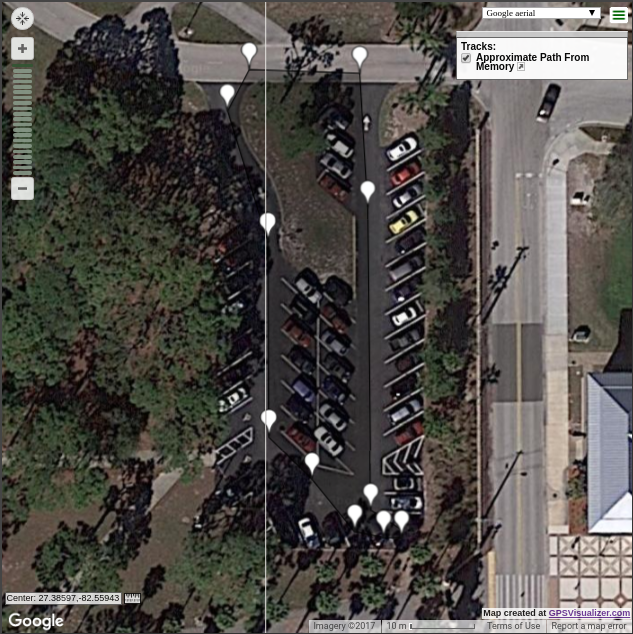
\includegraphics[height=0.45\textheight]{testRun/route_from_memory}
		\caption{Path Manually Mapped}
		\label{figRouteMemory}
	\end{subfigure}
	\begin{subfigure}{\textwidth}
		\centering
		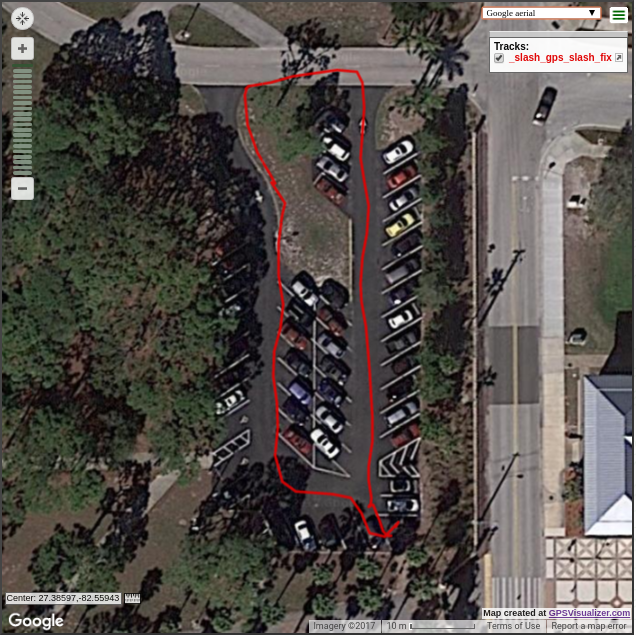
\includegraphics[height=0.4\textheight]{testRun/raw_gps_data}
		\caption{Path According to Phone's GPS}
		\label{figRouteGPS}
	\end{subfigure}
	
\end{figure}

\begin{figure}[p] 
	\caption{
		Filter Outputs For Different Sensor Fusions
	}
	\label{fig:ekfOutputs}
	\begin{subfigure}{\textwidth}
		\centering
		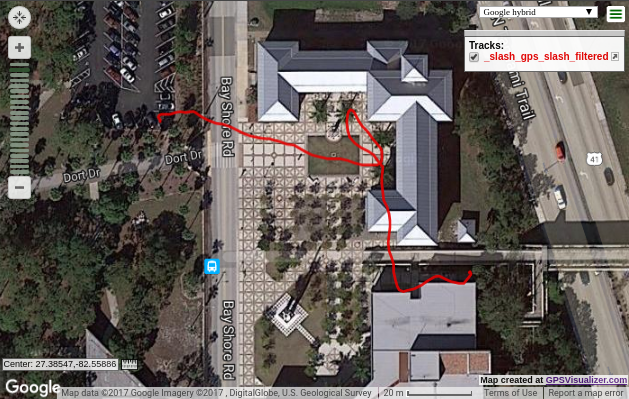
\includegraphics[height=0.4\textheight]{testRun/ekf_output_odom}
		\caption{Raw Wheel Odometry}
		\label{figRouteOdom}
	\end{subfigure}
	\begin{subfigure}{\textwidth}
		\centering
		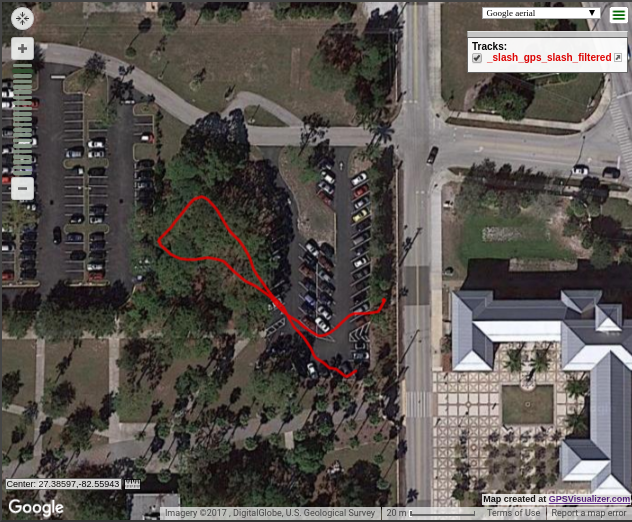
\includegraphics[height=0.4\textheight]{testRun/ekf_output_odom_imu}
		\caption{Wheel Odometry + IMU}
		\label{figRouteOdomImu}
	\end{subfigure}
	
\end{figure}

\begin{figure}[p] \ContinuedFloat
	\begin{subfigure}{\textwidth}
		\centering
		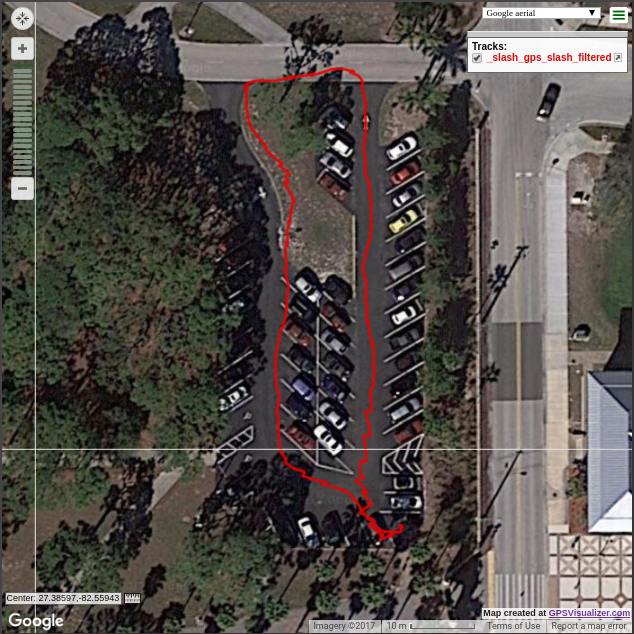
\includegraphics[width=\textwidth,height=\textheight,keepaspectratio]{testRun/ekf_output_odom_imu_gps}
		\caption{Wheel Odometry + IMU + GPS}
		\label{figRouteOdomImuGps}
	\end{subfigure}
\end{figure}